\chapter{Versuch}

Beim Versuch wurden Federn mit verschiedenen Federhärten mit verschiedenen Massen und verschiedenen Amplituden zum Schwingen gebracht. Mit einem Messwerterfassungssystem (CASSY) wurde die Auslenkung in Abhängigkeit von der Zeit aufgezeichnet.

Von den verschiedenen Federn wurde jeweils durch Messen der Auslenkung, die durch Massestücke verschiedener Masse hervorgerufen wird, die Federhärte bestimmt.

Anhand der Messswerte wurde
\begin{itemize}
    \item der Einfluss der Amplitude auf die Periodendauer
    \item der Zusammenhang $T \sim \sqrt{m}$
    \item der Zusammenhang $T \sim \frac{1}{D}$
\end{itemize}
untersucht.

Zusätzlich wurde anhand der aufgezeichneten Daten die schwingende Masse bestimmt, und mit der Masse des Massestücks verglichen.

Zu den Ergebnissen wurde jeweils eine Fehlerbetrachtung angestellt.

\section{Material}
\begin{itemize}
    \item Verschiedene Federn
    \item Massestücke bekannter Masse
    \item Stativmaterial
    \item CASSY mit Laptop und BMW-Box
    \item Faden und leichtes Gegengewicht
    \item Maßstab
\end{itemize}

\section{Aufbau}
Zunächst wurde mit dem Stativmaterial eine geeignete Befestigung für die Federn aufgebaut. Die Feder hängt oben an einem Haken, unten wird sie nicht befestigt, so dass sie frei schwingen kann. Neben der Feder wird der Bewegungs-Messwandler (BMW) angebracht. Das leichte Gegengewicht wurde an den Faden gebunden, dieser wurde über den BMW gelegt und sein anderes Ende an die Unterseite der Feder gebunden. Ebenfalls an die untere Seite der Feder wurde das Massestück angehängt.
Der BMW wird an das CASSY gesteckt, dieses wird an den Laptop angeschlossen.

Zur Messung der Federhärte wurde ebenfalls ein Stativ mit Haken aufgebaut, an den die Oberseite der Feder gehängt wurde, an die Unterseite wurden verschiedene Massestücke gehängt. Neben der Feder wurde ein Maßtab befestingt, um die Auslenkung der Feder ablesen zu können.

%TODO: Add images

\section{Durchführung}
\subsection{Bestimmung der Federhärte}
An die Feder wurden nach und nach Massestücke verschiedener Masse gehängt. Am Maßstab wurde jeweils die Auslenkung, also die Strecke, um die sich die Feder verlängert, wenn das Gewicht angehängt wurde, abgelesen und zusammen mit der Masse notiert.

\subsection{Aufzeichnen der Schwingung}
Die entsprechende Masse wurde an die Feder gehängt. Der BMW wurde in der Ruhelage des Feder-Masse-Systems auf Null gestellt. Dann wurde dass Massenstück nach unten ausgelenkt. Am CASSY konnte abgelesen werden, wie weit die Feder ausgelenkt wurde. Nachdem die gewünschte Auslenkung (und damit die Amplitude) eingestellt war, wurde die Feder losgelassen und möglichst schnell in CASSY die Aufzeichnung gestartet.

\section{Messergebnisse}
\subsection{Variieren der Masse}
\label{sub:change_mass}
Gemessen wurde jeweils mit einer Startauslenkung von $s_0 = \SI{3e-2}{\meter}$.

\begin{figure}[H]
\centering
\csvreader[tabular=rrrr, table head=Masse $m$ in \SI{}{\gram} & $\sqrt{m}$ & Periodendauer $T$ in \SI{}{\second} & Frequenz $f$ in \SI{}{\per\second} \\\hline]{data/spring1.csv}{}{\num{\csvcoli} & \num{\csvcolii} & \num{\csvcoliii} & \num{\csvcoliv}}
\caption{Messwerte mit verschiedenen Massen an Feder 1, $D = \SI{30.86 \pm 2.08}{\newton\per\meter}$}
\end{figure}

\begin{figure}[H]
\centering
\csvreader[tabular=rrrr, table head=Masse $m$ in \SI{}{\gram} & $\sqrt{m}$ & Periodendauer $T$ in \SI{}{\second} & Frequenz $f$ in \SI{}{\per\second} \\\hline]{data/spring2.csv}{}{\num{\csvcoli} & \num{\csvcolii} & \num{\csvcoliii} & \num{\csvcoliv}}
\caption{Messwerte mit verschiedenen Massen an Feder 2}
\end{figure}


\section{Auswertung}
\subsection{Bestimmung der Federhärten}
Aus den gemessenen Ausdehnungen kann mit dem Hook'schen Gesetz die Federhärte bestimmt werden.

\begin{align*}
F &= D \cdot s \\
D &= \frac{F}{s} \\
  &= \frac{m \cdot g}{s} \\
\end{align*}

Trägt man die Messwerte in ein Masse-Auslenkungs-Diagramm ein und bestimmt die Steigung der Ausgleichsgeraden, erhält man:
$$k = \frac{s}{m}$$

\begin{figure}[H]
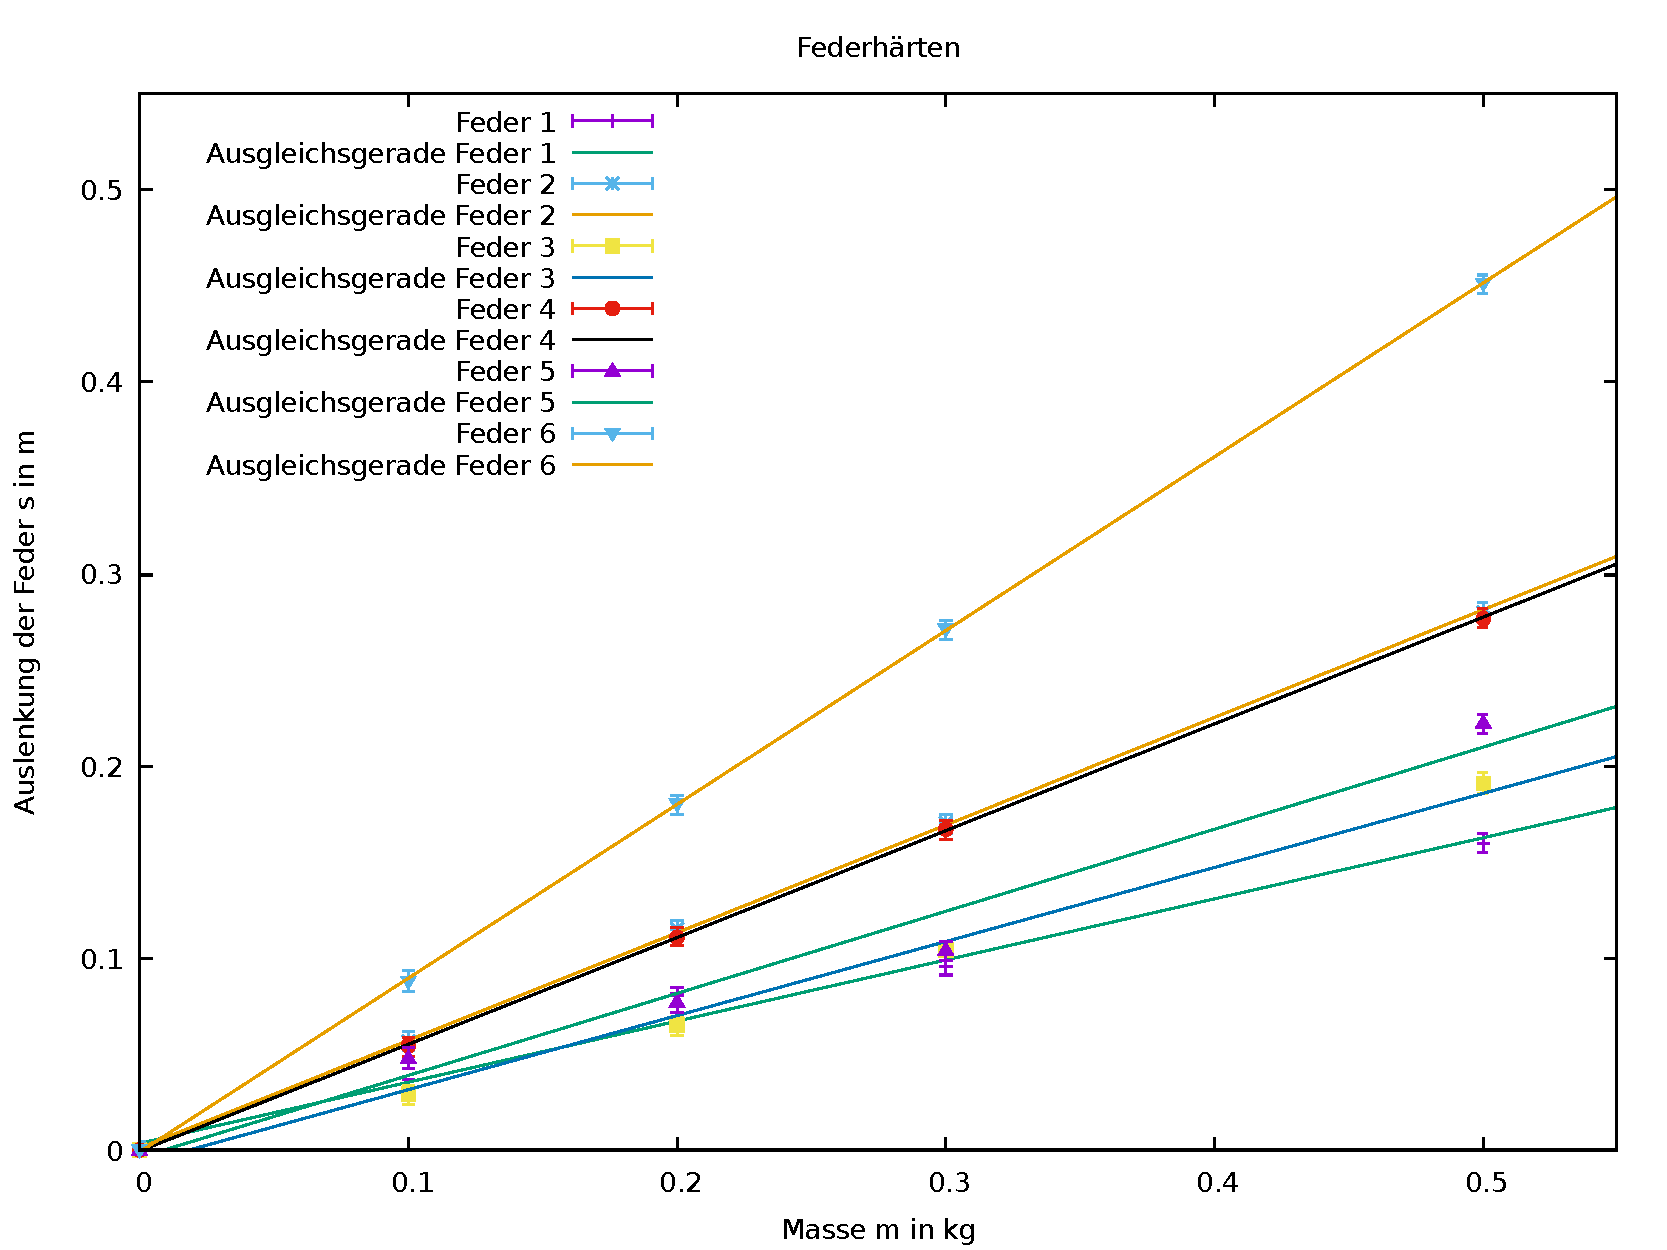
\includegraphics[width=\textwidth]{data/hardness.pdf}
\caption{Masse-Auslenkungs-Diagramm}
\end{figure}

Setzt man die Steigung in obige Gleichung ein, erhält man:
\begin{align*}
s &= k \cdot m \\
D &= \frac{m \cdot g}{k \cdot m} \\
  &= \frac{g}{k} \\
\end{align*}

\begin{figure}[H]
\centering
\begin{tabular}{lrrrr}
Feder & $k$ in \SI{}{\meter\per\kilo\gram} & Fehler $\Delta k$ in \SI{}{\meter\per\kilo\gram} & $D$ in \SI{}{\newton\per\meter} & Fehler $\Delta D$ in \SI{}{\newton\per\meter} \\ \hline
1 & \num{0.317} & \num{0.022} & \num{30.86} & \num{2.08}\\
2 & \num{0.560} & \num{0.004} & \num{17.52} & \num{0.12}\\
3 & \num{0.385} & \num{0.017} & \num{25.46} & \num{1.13}\\
4 & \num{0.556} & \num{0.003} & \num{17.66} & \num{0.07}\\
5 & \num{0.427} & \num{0.040} & \num{0.317} & \num{2.11}\\
6 & \num{0.904} & \num{0.003} & \num{10.85} & \num{0.03}\\
\end{tabular}
\end{figure}

Der Fehler der Steigung $\Delta k$ kann von GNUPlot ermittelt werden, indem der Fehler
$$\Delta s = \pm \SI{5e-3}{\meter}$$
angenommen wurde. Die Masse wurde als exakt angenommen.

$D$ ist durch ein Produkt (Faktor $\frac{1}{g}$) von $k$ abhängig, daher ist der relative Fehler gleich. (Der Ortsfaktor wird als exakt angenommen).

$$\Delta D = D \cdot \frac{\Delta k}{k}$$

Für den Ortsfaktor wurde der Wert
$$g = \SI{9.81}{\meter\per\square\second}$$
angenommen.

\subsection{Zusammenhang Periodendauer und Masse}
Für die Periodendauer gilt
$$T = 2\pi \frac{\sqrt{m}}{\sqrt{D}}$$
Damit gilt $T \sim \sqrt{m}$ mit der Proportionalitätskonstante
$$k = \frac{2\pi}{\sqrt{D}}$$

Aus den Messwerten (siehe \ref{sub:change_mass}) ergeben sich folgende Schaubilder:

\begin{figure}[H]
\centering
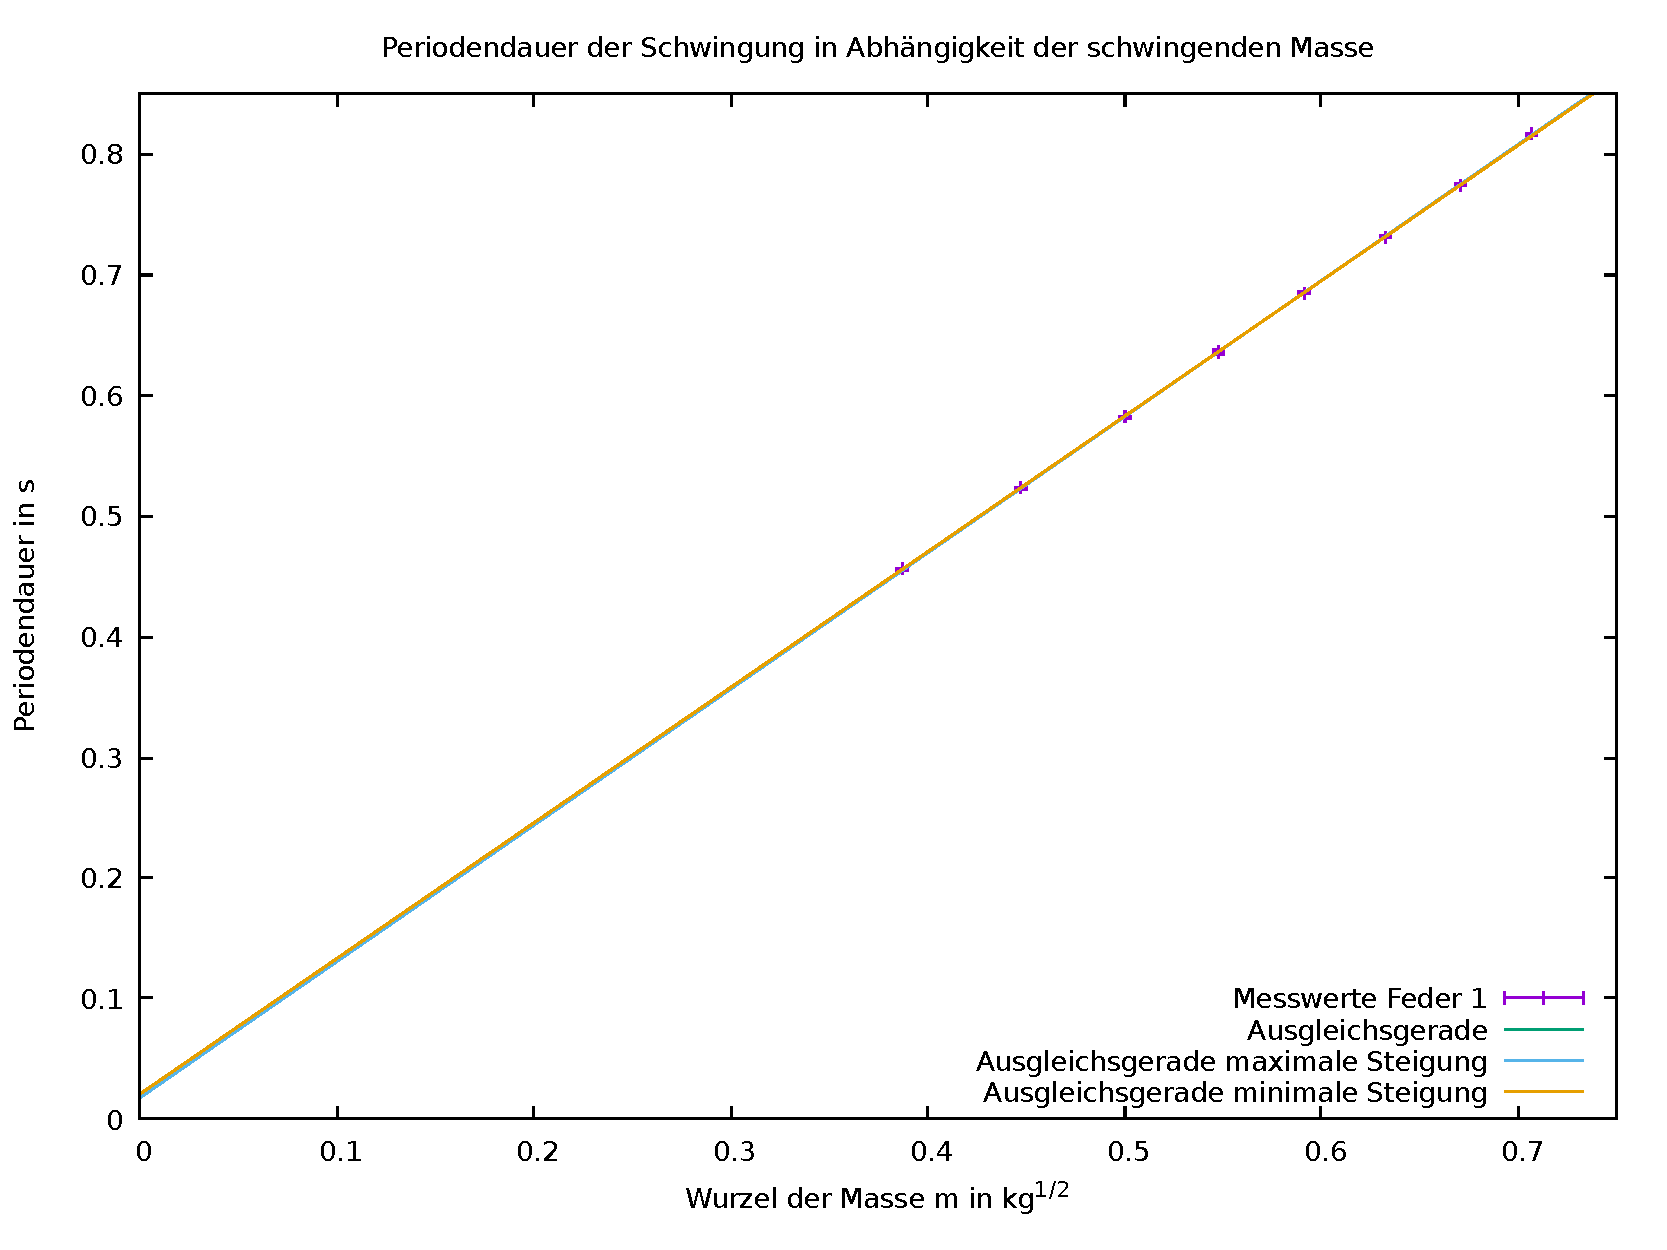
\includegraphics[width=0.8\textwidth]{data/spring1.pdf}
\caption{$\sqrt{m}$-$T$-Diagramm von Feder 1}
\end{figure}
\begin{figure}[H]
\centering
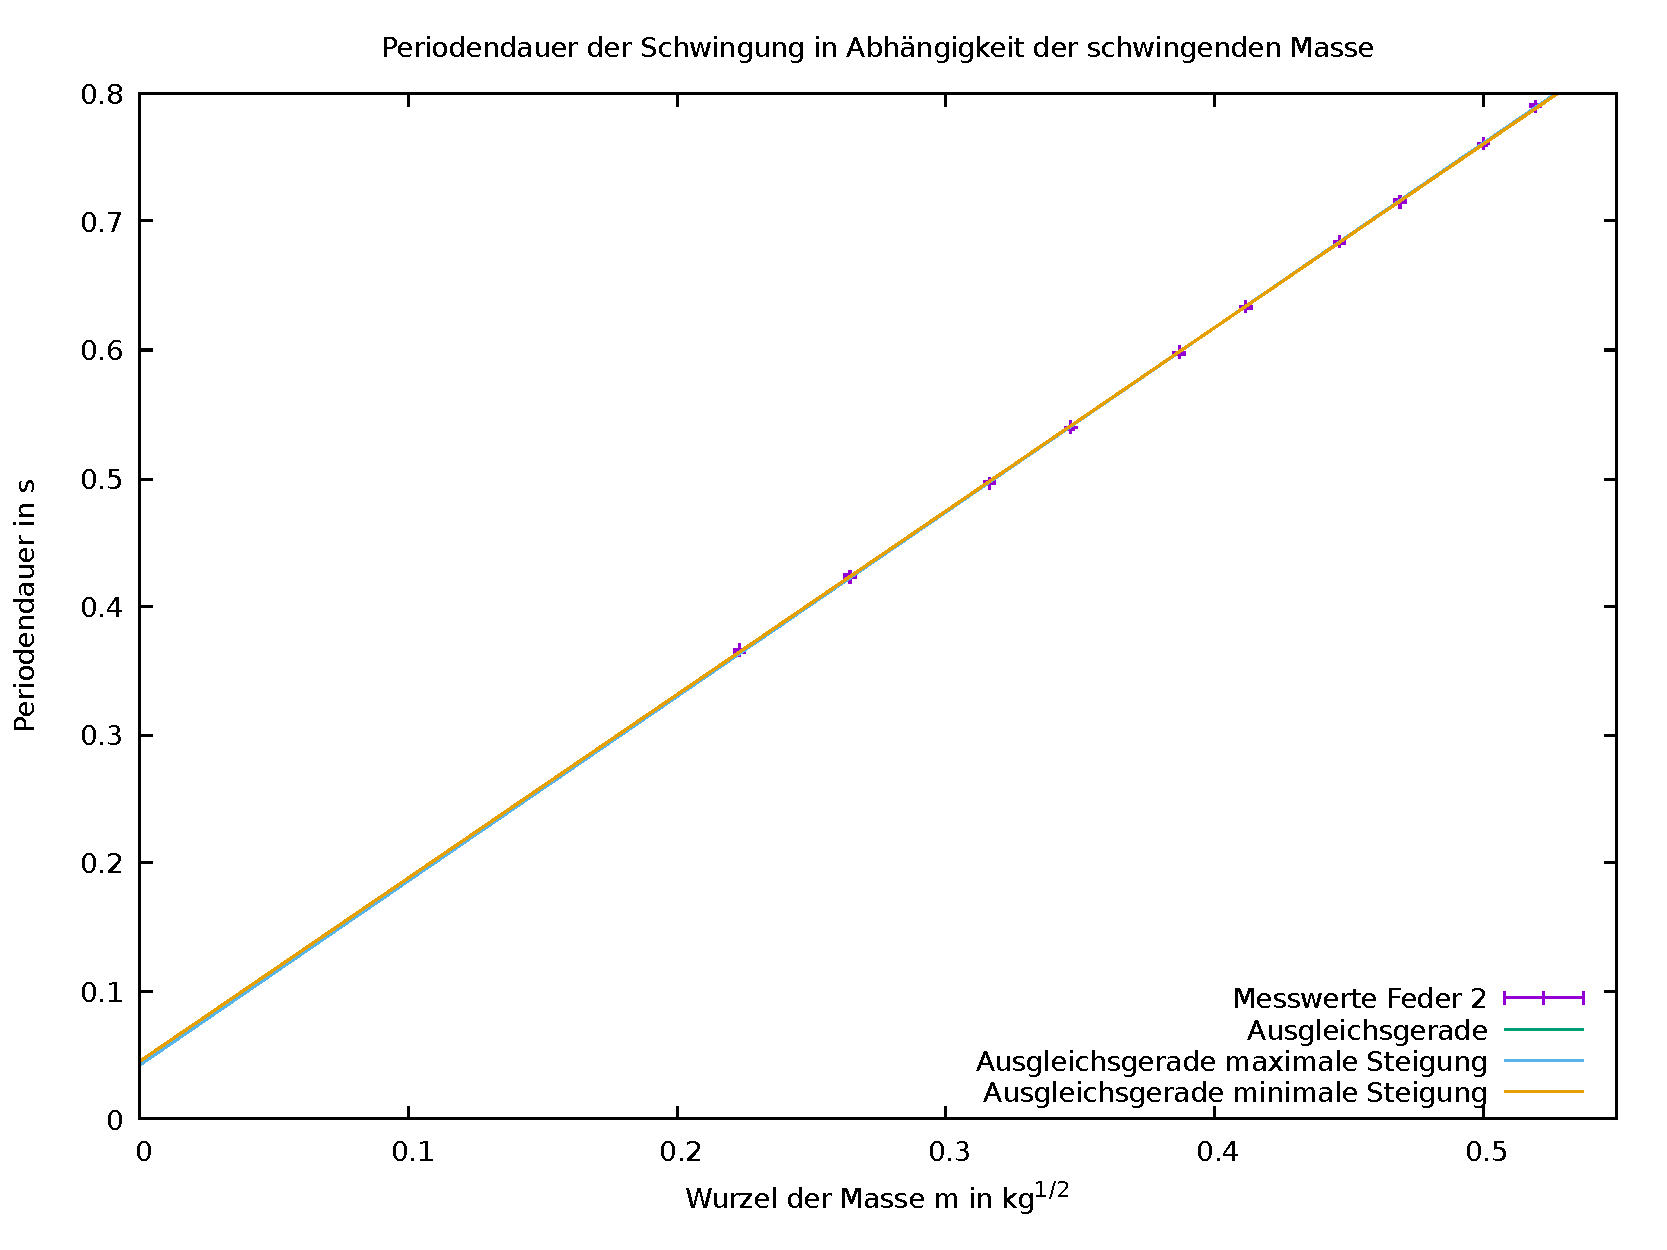
\includegraphics[width=0.8\textwidth]{data/spring2.pdf}
\caption{$\sqrt{m}$-$T$-Diagramm von Feder 2}
\end{figure}

In den Schaubildern sieht sich der $T \sim \sqrt{m}$ - Zusammenhang bestätigt.
GNUplot gibt den Fehler der Steigung mit unter $1\%$ an.

\subsection{Bestimmung der Federhärte aus dem funktionalen Zusammenhang}
Die Steigung des Graphen ergibt
$$k = \frac{T}{\sqrt{m}}$$

Setzt man sie in die Gleichung
$$T = 2\pi\sqrt{\frac{m}{D}}$$
ein erhält man:

\begin{align*}
\sqrt{m} &= \frac{T}{k} \\
T &= 2\pi\frac{T}{k \cdot \sqrt{D}} \\
\sqrt{D} &= \frac{2\pi}{k} \\
D &= \frac{4\pi^2}{k^2} \\
\end{align*}

Für den Fehler erhälkt man durch Ableiten der obigen Funktion für D:
$$\Delta D = \frac{8\pi^2}{k^3}\cdot \Delta k$$

\begin{figure}[H]
\centering
\begin{tabular}{r|rr|rr|rr}
 & $k$ in $\SI{}{\second\sqrt{\kilo\gram}^{-1}}$ & $\Delta k$ in $\SI{}{\second\sqrt{\kilo\gram}^{-1}}$ & $D$ in \SI{}{\newton\per\meter} & $\Delta D$ in \SI{}{\newton\per\meter} & $D_{D}$ in \SI{}{\newton\per\meter} & $\Delta D_{D}$ in \SI{}{\newton\per\meter} \\\hline
1 & \num{1.126} & \num{0.003} & \num{31.130} & \num{0.145} & \num{30.86} & \num{2.08} \\
2 &  \num{1.433} & \num{0.004} & \num{19.214} & \num{0.097} & \num{17.52} & \num{0.12}
\end{tabular}
\caption{Ermittelte Werte für $D$, sowie Vergleich mit direkt gemessener Federhärte $D_D$}
\end{figure}

Die errechnete Steigung liegt bei Feder 1 im Bereich des Messfehlers, bei Feder 2, jedoch nicht. Eine Ursache dafür könnte ein in der Fehlerrechnung nicht berücksichtigter systematischer Fehler, oder ein Falsch abgeschätzter Messfehler sein.

\subsection{Zusammenhang Periodendauer und Federhärte}
Für die Periodendauer gilt
$$T = 2\pi \frac{\sqrt{m}}{\sqrt{D}}$$
Damit gilt $T \sim \frac{1}{\sqrt{D}}$ mit der Proportionalitätskonstante
$$k = 2\pi\sqrt{m}$$

Aus den Messwerten (siehe \ref{sub:change_hardness}) ergeben sich folgende Schaubilder: